\documentclass[11pt]{article}


\usepackage[sort]{natbib}
\usepackage{bm,amsmath,bbm,amsfonts,nicefrac,latexsym,amsmath,amsfonts,amsbsy,amscd,amsxtra,amsgen,amsopn,bbm,amsthm,amssymb,graphicx, subfig}
\usepackage{wrapfig, caption, subcaption}
\usepackage{fancyhdr}
\usepackage[margin=1.0in]{geometry}




\title{Third Monitoring Committee Meeting\\\vspace{4mm} \normalsize{Understanding the Information Content in Diverse Observations of Forest Carbon Stocks and Fluxes for Data Assimilation and Ecological Modeling\\ NERC case partnership with Forest Research}}
\date{\normalsize{3$^{\text{rd}}$ December 2014, \ Maths Room 100}}
\author{\normalsize{E. Pinnington}}


\newtheorem{theorem}{Theorem}[section]
\newtheorem*{defn}{Definition}



	
\begin{document}

\maketitle

\section{Introduction}

In our last monitoring committee the Data Assimilation Linked Ecosystem Carbon model (DALEC) \cite{williams2005improved} was introduced and we showed how this model could be implemented in a variational data assimilation (DA) framework in order to look at the information content of different forest carbon balance observations. In particular, Shannon Information Content \cite{rodgers2000inverse} was used to investigate the level of information provided by single and successive observations of Net Ecosystem Exchange (NEE) and it was shown that observations of NEE taken in summer with warmer temperatures and higher daily irradiances had a higher information content than those taken in winter with lower temperatures and lower daily irradiance. This makes physical sense as observations of NEE in the summer are of greater magnitude and give more information about the fluxes of carbon throughout the forest. The error in our linearized version of DALEC was also considered in the last report, this is important as in four-dimensional variational data assimilation (4D-Var) the linearized model is used in the tangent linear hypothesis, the results from this experiment showed the linearized DALEC to perform poorly. However since the last report I have found that the linear DALEC was not derived correctly and repeating these experiments shows the tangent linear hypothesis to be a good approximation for DALEC. 

Since our last meeting I have continued the work on the information content of forest carbon balance observations. I have looked at the degrees of freedom for signal as another measure for information content and have written a first draft of a report on my findings (I have included this alongside my monitoring report). I have built DALEC into a 4D-Var scheme assimilating data from a young pine stand in Oregon in order to estimate the five carbon pools which make up the state vector for DALEC. I have started visiting the Forest Research site at Alice Holt on a weekly basis and am helping with current measurement campaigns. A new version of the DALEC model has been released since our last meeting (DALECV2 \cite{Bloom2014}) which can be parameterized for both evergreen and deciduous forests, I have started working with this model now as the research site at Alice Holt is largely deciduous and the previous DALEC with which I have been working only models evergreen forests. Currently, I have coded my own version of DALECV2 in Python and have built this into a 4D-Var scheme similar to that which I had written for the state estimation with DALEC but now estimating the 17 model parameters as well as the initial value for the carbon pools. I hope this will allow me to parameterize DALECV2 for the Alce Holt research site. In this report we begin by showing some of the results from the information content experiments.

\section{Information Content}

In the last monitoring report the Shannon Information Content (SIC) was used as a measure of the reduction in entropy of a system given a set of observations \cite{stewart2008correlated}. The SIC can be derived as,
\begin{equation} \label{sic}
\text{SIC}=\frac{1}{2}\text{ln}\frac{\begin{vmatrix} \textbf{B} \end{vmatrix}}{\begin{vmatrix} \textbf{A} \end{vmatrix}},
\end{equation}
where $\begin{vmatrix} \textbf{B} \end{vmatrix}$ is the determinant of the background error covariance matrix and $\begin{vmatrix} \textbf{A} \end{vmatrix}$ is the determinant of the analysis covariance matrix. The NEE of a forest in the DALEC model is expressed as the difference between the Gross Primary Production (GPP) of the forest and the respirations of the forest at time $t$,
\begin{equation} \label{nee}
\text{NEE}(t)=-(1-p_2)\text{GPP}(C_f(t),\phi)+p_8C_lT(t)+p_9C_sT(t),
\end{equation}
where $p_2, p_8, p_9$ are model parameters, $C_f, C_l, C_s$ are carbon pools, $\phi$ represents the meteorological driving data used by the GPP function and $T=\frac{1}{2}\text{exp}(\Theta T_{\text{mean}}(t))$ is an exponential function of the mean daily temperature. Combining equations \ref{sic} and \ref{nee} and using the 4D-Var framework for DALEC we can derive the SIC for an observation of NEE at time $t$ as,
\begin{equation}
\text{SIC for NEE}(t)=\frac{1}{2}\text{ln}\frac{(p_{2}-1)^{2}\text{GPP}'^{2}(C_f(t), \phi)\sigma_{cf,b}^{2}+\sigma_{nee,o}^{2}+T^2(t)(p_{9}^2\sigma_{cs,b}^2+p_8^2\sigma_{cl,b}^2)}{\sigma_{nee,o}^{2}}.
\end{equation}
where $\sigma_{cf,b}^{2}, \sigma_{cl,b}^2, \sigma_{cs,b}^2$ are the background variances for the carbon pools and $\sigma_{nee,o}^{2}$ is the variance for an observation of NEE. If we assume that the variances and parameters here are fixed, we can see that the size of the $SIC$ is dependent on the temperature term, $T(t)$, and the square of the first derivative of $GPP$. Generally, the value of $GPP$ (and its first derivative) is highest in summer with higher temperatures and higher total daily irradiance. We therefore have that there will be more information content in observations that are taken when temperatures are higher. Physically this makes sense as more $NEE$ takes place when temperatures are higher (to a point), so measurements are of greater magnitude and give us more information about carbon fluxes. 

By plotting the $SIC$ for a single observation of $NEE$, varying with three years of meteorological driving data, next to the temperature term ($T(t)$) for the same data we can see that both are closely linked, figure \ref{fig:SICNEET}.
\begin{figure}[ht]
\centering
\subfigure{
  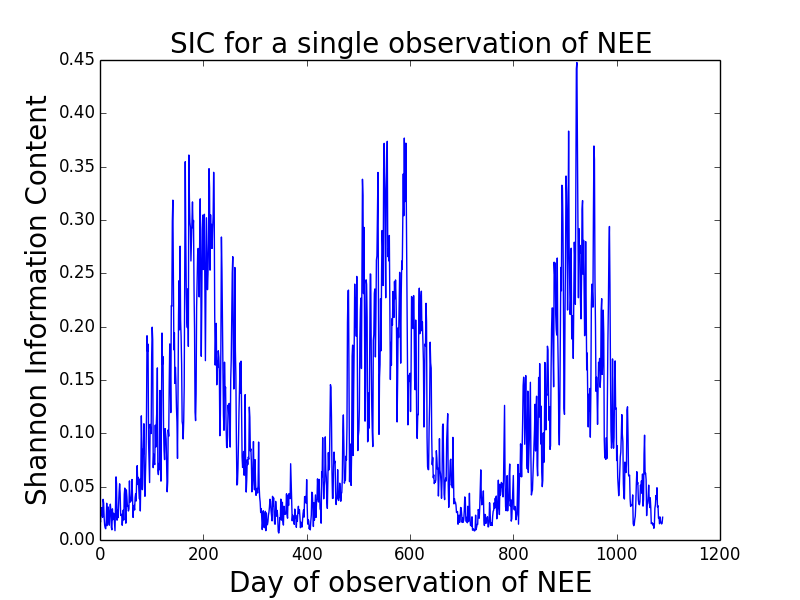
\includegraphics[width=.46\linewidth]{SIC1Obs_0_1095.png}
  %\caption{$SIC$ for a single observation of $NEE$.}
  \label{fig:sub1}
}
\subfigure{
  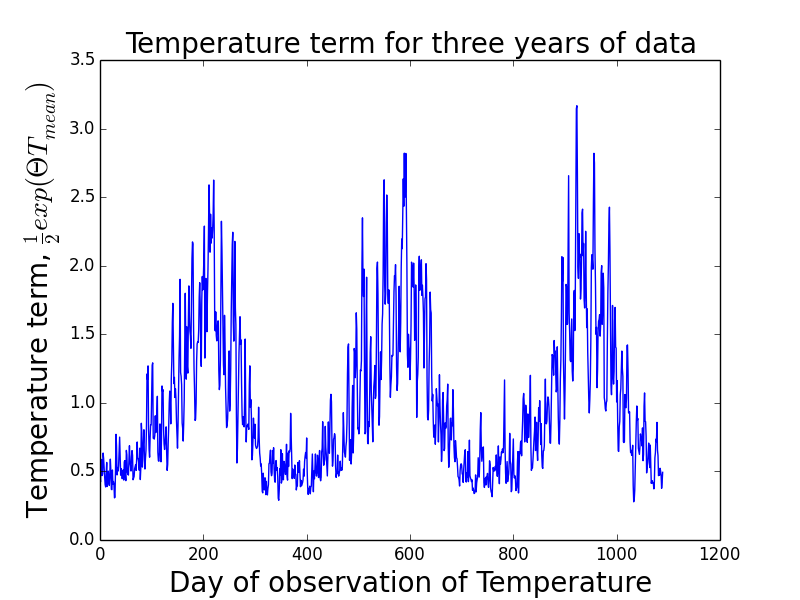
\includegraphics[width=.46\linewidth]{Temp_0_1095.png}
  %\caption{Temperature term, $\frac{1}{2}exp(\Theta  T_{mean})$.}
  \label{fig:sub2}
}
\caption{SIC and temperature varying over three years using driving data from Oregon pine forest.}
\label{fig:SICNEET}
\end{figure}
This shows that observations of $NEE$ made in the summer are much more valuable than those made in the winter assuming warmer temperatures, higher daily irradiance and a higher amount of foliar carbon in the summer.

In the report this idea is also explored for the degrees of freedom for signal (DFS) measure for information content. The DFS indicates the number of elements of the state that have been measured by the observations. If we consider a state vector $\textbf{x}$ with $n$ elements (or $n$ degrees of freedom) then the maximum value the DFS could obtain would be $n$, in this case all elements of the state would have been measured. Conversely if DFS $= 0$ then no elements of the state would have been measured by our observations \cite{fowler2011measures}.The DFS can be written as,
\begin{equation}
\text{DFS} = n - \text{trace}(\mathbf{B}^{-1}\mathbf{A}).
\end{equation}

The result in figure \ref{fig:SICNEET} can be reproduced using the DFS showing that we measure more elements of our state with observations of NEE made in summer than observations made in winter. To understand how much more value the summer observations of NEE have compared to the winter observations we have plotted the increasing SIC and DFS for 50 observations made from December $21^{\text{st}}$ onwards and also the the constant line of SIC and DFS for one observation of $NEE$ made in summer at a mean daily temperature of $26^{o}\text{C}$ on July $12^{\text{th}}$. This is shown in figure \ref{sicdfs}.

\begin{figure}[ht]
\centering
  \begin{subfigure}
  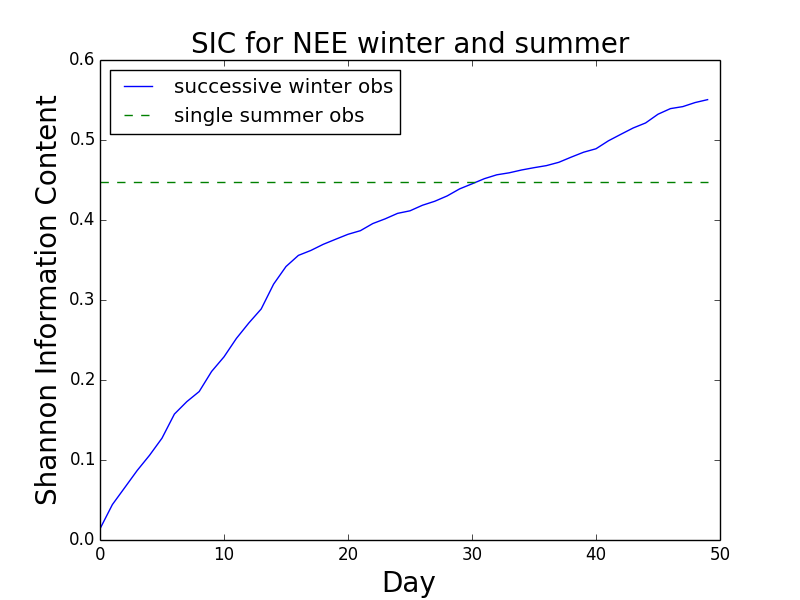
\includegraphics[width=.49\linewidth]{succwinter_singlesummer.png}
  %\caption{$SIC$ for a single observation of $NEE$.}
  \label{fig:sub1}
  \end{subfigure}%
  \begin{subfigure}
  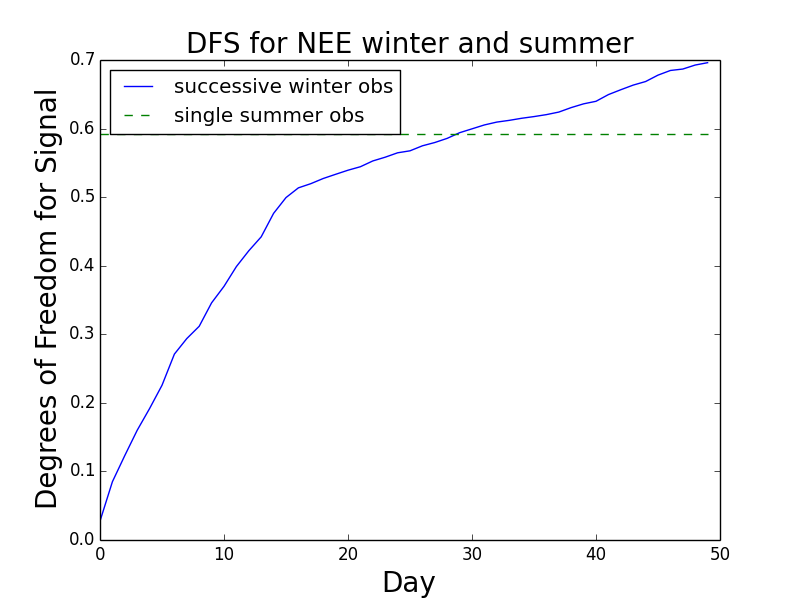
\includegraphics[width=.49\linewidth]{succwinter_singlesummerdofs.png}
  %\caption{Temperature term, $\frac{1}{2}exp(\Theta  T_{mean})$.}
  \label{fig:sub2}
  \end{subfigure}
\caption{SIC (left) and DFS (right) for a single summer observation of NEE and successive winter observations of NEE using driving data from Oregon pine forest.}
\label{sicdfs}
\end{figure}
Figure \ref{sicdfs} shows us that, for the driver data used in this experiment, we require 31 days of NEE observations to gain the same reduction in entropy for our analysis as 1 observation made in the summer and 30 days of NEE observations to achieve the same DFS as 1 observation made in the summer. For more detail on the information content experiments with DALEC please see the attached report \cite{pinningtoninfocon}.

\section{4D-Var with DALEC}

In 4D-Var we aim to maximise the probability of our initial state $\textbf{x}_0$ given a set of observations $\textbf{y}$, $P(\textbf{x}_0|\textbf{y})$, over some time window, $N$.  $P(\textbf{x}_0|\textbf{y})$ is maximised by minimising a cost function $J(\textbf{x})$ derived from Baye's Theorem \cite{lewis2006dynamic}. The cost function is given as,

\begin{equation}
J(\textbf{x}_0) = \frac{1}{2}(\textbf{x}_0-\textbf{x}_b)^{T}\textbf{B}^{-1}(\textbf{x}_0-\textbf{x}_b)+\frac{1}{2}\sum_{i=0}^{N}(\textbf{y}_i-h_i(\textbf{x}_i))^{T}\textbf{R}_{i}^{-1}(\textbf{y}_i-h_i(\textbf{x}_i)),
\end{equation}•
where $\textbf{x}_b$ is our background and acts as our initial guess to our state $\textbf{x}_0$, $\textbf{B}$ is the background error covariance matrix and quantifies our knowledge of the error in our background, $h_i$ is our observation operator at time $t_i$ and maps our state vector evolved by our nonlinear model ($m_{0\rightarrow i}(\mathbf{x}_{0})=\textbf{x}_i$) to the observations at this time $\textbf{y}_i$ and $\textbf{R}_i$ is the observation error covariance matrix and represents our knowledge of the uncertainty in the observations. The state that minimises the cost function is called the analysis and is denoted as $\textbf{x}_a$, this state is found using a minimisation routine that takes the cost function, our initial guess ($\textbf{x}_b$) and also the gradient of the cost function defined as,

\begin{equation}
\nabla J(\textbf{x}_0) = \textbf{B}^{-1}(\textbf{x}_0-\textbf{x}_b)-\sum_{i=0}^{N}\textbf{M}_{i,0}^{T}\textbf{H}_i^{T}\textbf{R}_{i}^{-1}(\textbf{y}_i-h_i(\textbf{x}_i)),
\end{equation}•
where $\textbf{H}_i = \frac{\delta h_i(\textbf{x}_i)}{\delta\textbf{x}_i}$ is our linearized observation operator and $\mathbf{M}_{i,0}=\mathbf{M}_{i-1}\mathbf{M}_{i-2}\cdots\mathbf{M}_0$ is our tangent linear model with $\mathbf{M}_i=\frac{\delta m_{i}(\textbf{x}_{i})}{\delta \textbf{x}_{i}}$.

For DALEC our state $\textbf{x}_0$ corresponds to the initial values of the five carbon pools,  $\textbf{x}_0 = (C_f(t_0), C_r(t_0), C_w(t_0), C_l(t_0), C_s(t_0))^T$. We can calculate the linearized model for DALEC as,
\begin{equation}
\mathbf{M}_{i}= 
\begin{pmatrix} 
(1-p_5)+p_3(1-p_2)\zeta_i & 0 & 0 & 0 & 0 \\
p_4(1-p_3)(1-p_2)\zeta_i & (1-p_7) & 0 & 0 & 0 \\
(1-p_4)(1-p_3)(1-p_2)\zeta_i & 0 & (1-p_6) & 0 & 0 \\
p_5 & p_7 & 0 & (1-(p_1+p_8)T_i) & 0 \\
0 & 0 & p_6 & p_1T_i & (1-p_9T_i) \\
\end{pmatrix}, \label{linmod}
\end{equation}
where $\zeta_i = \text{GPP}'(C_f(t_i), \phi)$ and $T_{i}=T(t_i)$. The cost function and gradient of the cost function were coded in Python along with the DALEC model. Meteorological driving data and observations for assimilation were initially taken from a young pine forest in Oregon. Our analysis ($\textbf{x}_a$) was found by passing our cost function and its gradient function along with $\textbf{x}_b$ to the Broyden-Fletcher-Goldfarb-Shanno minimization algorithm (BFGS) \cite{Nocedal1999} found in the scipy.optimize package for Python.  The results for our analysis when assimilating a years worth of NEE observations can be seen in figure \ref{4dvardalec}.

\begin{figure}[ht]
\centering
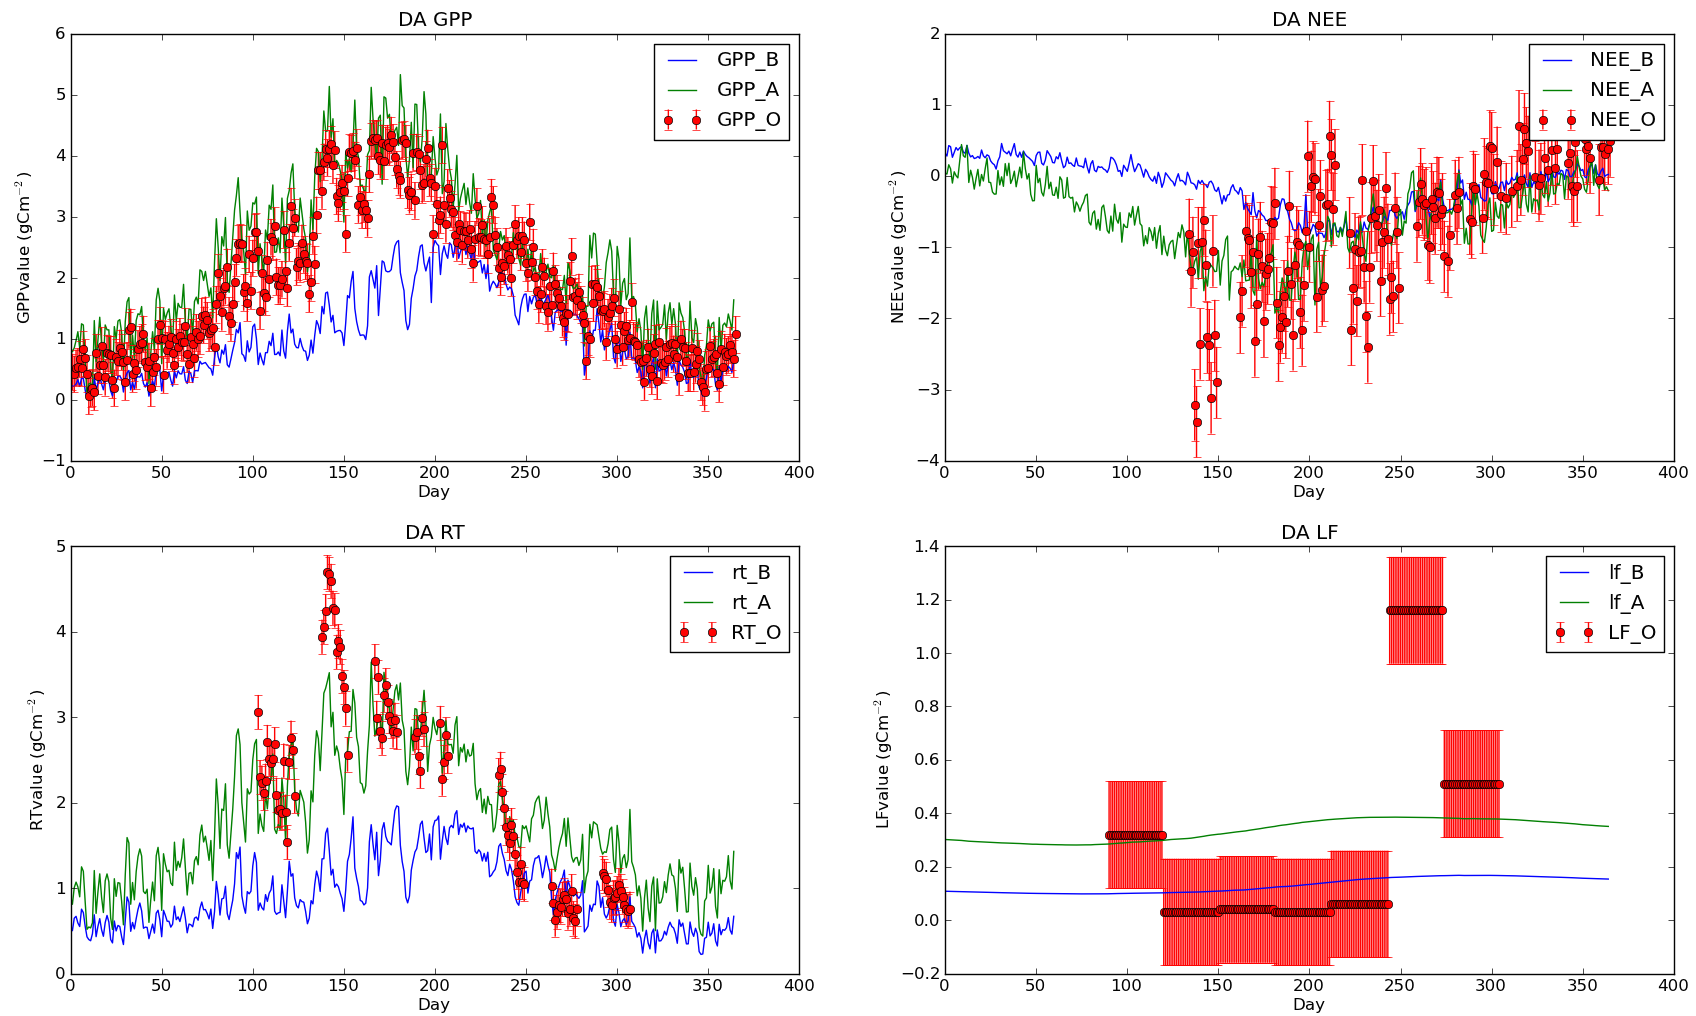
\includegraphics[height=.55\textwidth, ]{dacodeneeonly.png}
\caption{4D-Var with DALEC assimilting observations of NEE over a year from Oregon pine stand. Here the blue line is our $\textbf{x}_b$ run forward, the green line is our $\textbf{x}_a$ run forward and the red dots are diferent forest carbon balance observations corresponding to GPP (top left), NEE (top right), total respiration (RT) (bottom left) and litter fall (LF) (bottom right).}
\label{4dvardalec}
\end{figure}
In figure \ref{4dvardalec} we can see a better fit to the observations after assimilation of the NEE observations when our $\textbf{x}_a$ is run forward in figure \ref{4dvardalec}. Assimilating the NEE data not only improves the fit of the model trajectory to the observations of NEE but also to the observations of GPP and total respiration (RT). This shows that by assimilating NEE observations we are also gaining information about GPP and RT. This is expected as NEE is a product of RT and GPP (NEE = RT - GPP) so improving our estimate of NEE should also improve our estimate of RT and GPP. We can also see how simple the DALEC model is in some areas by looking at its prediction of litter fall (LF) which is just modelled as a constant multiplied by $C_f$ in this evergreen version of DALEC.

More experiments had been planned with DALEC in a 4D-Var scheme however with the release of DALECV2 \cite{Bloom2014} it was decided that it would be best to begin working with this new model. This new model DALECV2 can be paramterized for either deciduous or evergreen forests where as the DALEC being used for previous experiments only models evergreen forests. Paramterizing the model for a deciduous forest is important as the Forest Research site at Alice Holt forest is mainly decidous and this is where I will be based for my field work.

\section{Current Work}
\begin{wrapfigure}{R}{0.25\textwidth}
    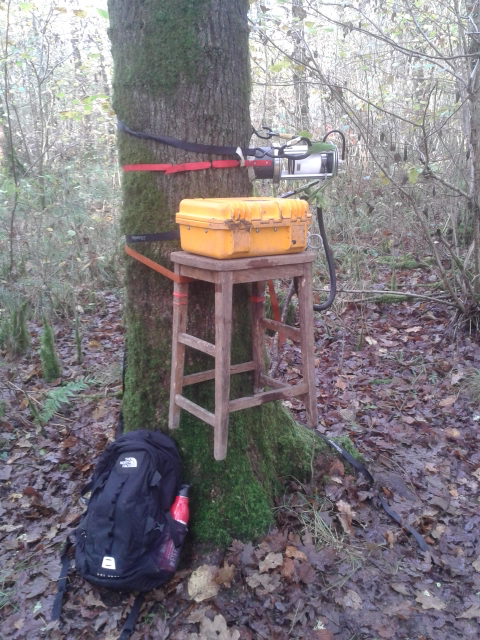
\includegraphics[width=0.25\textwidth]{treechamber.png}
  \caption{Tree respiration chamber used at Alice Holt research site.}
\label{stem}
\end{wrapfigure}
I am currently working on getting DALECV2 coded up with a 4D-Var scheme in Python with a state made up of the initial carbon pool values and the 17 model parameters so that the model can be parameterized for the Alice Holt research site.
I have started to work with meteorological driving data and forest carbon balance observations from Alice Holt and am converting this data into the correct format to be used with the DALECV2 model. 

I have recently started working at Forest Research once a week on Tuesdays. I am currently helping out conducting stem and soil respiration measurements, the equipment used for the stem respiration measurements can be seen in figure \ref{stem}. These measurements form part of an existing measurement campaign that Forest Research are conducting. The measurements of stem respiration may not be directly used in my own work, however they are valuable for my understanding of conducting fieldwork measurements and learning my way around the Straits enclosure where the bulk of the carbon balance measurements are made at the Alice Holt site.





\section{Future Plans}

I shall continue to work on parameterizing DALECV2 for the Alice Holt research site. I also plan on repeating the information content experiments with DALECV2 to see if we have similar results as achieved with the original DALEC model.


\section{Professional and Academic Development}

\subsection{Masters Courses}
Since our last meeting I have now received the grades for my final three assessed modules:
\begin{itemize}
\item MTMG49 (Boundary Layer) - 72\%
\item MTMD01 (Environmental Data Visualization) - 78\%
\item MTMD02 (Operational Data Assimilation) - 70\%
\end{itemize}

\subsection{Transferable Skills}

During my PhD I have taken part in the following courses:
\begin{itemize}
\item 28/01/2014 - Basic Statistics Refresher - RRDP

\item 31/03/2014-01/04/2014 - Land Data Assimilation workshop at UCL - ESA

\item 23/04/2014-25/03/2014 - Correlated Observation Errors in Data Assimilation - ESA

\item 13/05/2014 - Social Media - Bloggs, Twitter and Your Online Presence - RRDP

\item 29/05/2014 - How to Write a Paper - RRDP

\item 25/06/2014-26/06/2014 - Software Carpentry - Git and Python

\item 10/07/2014-11/07/2014 - Forest Research - Helped with field work LiDAR 

\item 29/09/2014-03/10/2014 - NERC course - Software Developement for Environmental Scientists

\item 08/10/2014-10/10/2014 - Environment YES - NERC competition at Syngenta, Jesops Hill
\end{itemize}

I have also demonstrated on the NERC 'Data assimilation and visualization for environmental sciences' course held from 15/09/2014 to 19/09/2014 organised by Dr. Amos Lawless.

On 17/12/14 I will be giving a presentation at the Mathematics for Planet Earth industry day at Imperial College about my project and working with a case partner.

\subsection{Summer School}
I attended the Fluxcourse summer school held at the University of Colorado from 21/07/2014 to 01/08/2014. During the course we stayed at the University's mountain research station near Boulder, Colorado. The course covered many different aspects of measuring and modelling the CO$_2$ flux of forests and plants. I found spending time with other early career scientists studying similar problems very helpful in the understanding of my own research topic. At the end of the course we had to present a piece of group work using a carbon balance model with a data assimilation scheme.


\bibliography{../../phdref}{}
\bibliographystyle{plain}
\end{document}